\documentclass[10pt]{article}
\renewcommand{\baselinestretch}{1.8}

\usepackage[a4paper,left=0.8in,right=0.8in,top=1.1in,bottom=1.1in]{geometry}
\usepackage{tikz-qtree}
\usepackage{algorithm}
\usepackage{algpseudocode}
\makeatletter
\renewcommand{\ALG@beginalgorithmic}{\footnotesize}
\makeatother
\usepackage{graphicx}
\usepackage{subcaption}

\usepackage{multicol}
\setlength\columnsep{24pt}

\algnewcommand\algorithmicforeach{\textbf{for each}}
\algdef{S}[FOR]{ForEach}[1]{\algorithmicforeach\ #1\ \algorithmicdo}

\algdef{S}[FUNCTION]{Function}
   [3]{{\keywordfont #1} \textproc{\texttt{#2}}\ifthenelse{\equal{#3}{}}{}{\texttt{(#3)}}}
  
\algdef{E}[FUNCTION]{EndFunction}
   [1]{\algorithmicend\ \texttt{\textproc{#1}}}

\algrenewcommand\Call[2]{\texttt{\textproc{#1}\ifthenelse{\equal{#2}{}}{}{(#2)}}}
   
\newcommand\keywordfont{\sffamily\bfseries}
\algrenewcommand\algorithmicend{{\keywordfont end}}
\algrenewcommand\algorithmicfor{{\keywordfont for}}
\algrenewcommand\algorithmicforeach{{\keywordfont for each}}
\algrenewcommand\algorithmicdo{{\keywordfont do}}
\algrenewcommand\algorithmicuntil{{\keywordfont until}}
\algrenewcommand\algorithmicfunction{{\keywordfont function}}
\algrenewcommand\algorithmicif{{\keywordfont if}}
\algrenewcommand\algorithmicthen{{\keywordfont then}}
\algrenewcommand\algorithmicelse{{\keywordfont else}}
\algrenewcommand\algorithmicreturn{{\keywordfont return}}

\title{Wait-free Queues with Polygarithmic Step Complexity}
\date{\today}

\usepackage{amsmath,amssymb,amsthm}
\newtheorem{theorem}{Theorem}
\newtheorem{lemma}[theorem]{Lemma}
\theoremstyle{definition}
\newtheorem{definition}{Definition}

\begin{document}
\maketitle

%\begin{abstract}
%This is the paper's abstract \ldots
%\end{abstract}

\section{Previous Work}
\begin{table}[hbt]
  \begin{center}
  \begin{tabular}{l|c|c|c}
    & Type & Progress Property  & Complexity \\ \hline
    MichaelS96~\cite{DBLP:conf/podc/MichaelS96} & Singly Linked List & Lock-free & $\Omega(p)$ \\ \hline
    MoirNSS05~\cite{DBLP:conf/spaa/MoirNSS05} & Linked List with Elemination & & \\ \hline
    HoffmanSS07~\cite{DBLP:conf/opodis/HoffmanSS07} & Linked List with Baskets & & $\Omega(p)$ \\ \hline
    Ladan-MozesS08 ~\cite{DBLP:journals/dc/Ladan-MozesS08} & Doubly linked list & Lock-free & $\Omega(p)$ \\ \hline
    MilmanKLLP18~\cite{DBLP:conf/spaa/MilmanKLLP18} & Linked List with batching same type ops & Lock-free & \\ \hline
    GidenstamST10~\cite{DBLP:conf/opodis/GidenstamST10} & Linked list of arrays & Lock-free & $\Omega(p+len(array))$ \\ \hline
    KoganP11~\cite{DBLP:conf/ppopp/KoganP11} &  Linkedlist with head and tail pointers & Wait-free & $\textsc{O}(p\times\text{bakery-max})$
  \end{tabular}
  \caption{Linearizable ME-MD Queus}
  \end{center}
\end{table}

\section{ Universal Construction using Tournament Tree with Big CAS Objects }
\paragraph{}
Jayanti~\cite{DBLP:conf/podc/Jayanti98a} proved an $\Omega(\log p)$ lower bound on the worst-case shared-access time complexity of $p$-process universal constructions. He also introduced~\cite{DBLP:conf/podc/ChandraJT98} a construction that achieves $\textsc{O}(\log^2 p)$ shared accesses. Here, we first introduce a universal construction using $\textsc{O}(\log p)$ CAS operations~\cite{DBLP:conf/fsttcs/JayantiP05}. We use the universal construction as a stepping stone towards our queue algorithm, so we will not explain it in too much detail.
\paragraph{}
We introduce our universal construction in Algorithm~\ref{alg1} with a tournament tree with $p$ leaves and height $\log(p)$ is shared among $p$ processes. Nodes are CAS objects, and each leaf is assigned to one process exclusively. Each CAS object stores a sequence of operations. When process $P_i$ wishes to apply an operation $op$ on the implemented object, it appends $op$ to its assigned leaf and tries to propagate it up to the root. The sequence of operations stored in Node $n$'s CAS object shows the order of the operations propagated up to $n$.
The history of operations stored at the root is the linearization ordering. The operation $op$ is linearized when it is appended to the root.

\begin{center}
\Tree [ [ [ $P_1$ $P_2$ ] [ $P_3$ $P_4$ ] ]
          [ [ $P_5$ $P_6$ ] [ $P_7$ $P_8$ ] ] ]
\end{center}


Leaf $l_i$ stores the sequence of the operations invoked by $P_i$. 
The algorithm uses a subroutine \textsc{Refresh}($n$) that concatenates new operations from node $n$'s children (that have not already been propagated to $n$) to the sequence of operations stored in $n$ and tries to CAS the new sequence into $n$. In other words, \textsc{Refresh}($n$) tries to append $n$'s children's new operations to $n$'s sequence.
After a process adding a new operations to its leaf, it has to propagate new operations up to the root. \textsc{Propagate}($n$) tries to append $n$'s new operations to the root $n$ by recursively calling \textsc{Refresh}($n$). In each step if a \textsc{Refresh}($n$) fails, it means another CAS operation has succeeded; if so, it tries to \textsc{Refresh}($n$) again. If the second attempt fails too, another process has already appended the operations the current \textsc{Propagate} is trying to append.
Operations that were in $l_i$ before \textsc{Propagate}($l_i$.parent) was invoked are guaranteed to be added to the root by the time the \textsc{Propagate}($l_i$.parent) finishes.



\begin{figure}

\begin{center}


\begin{subfigure}[b]{.49\textwidth}


  \centering
  \resizebox{\columnwidth}{!}{
  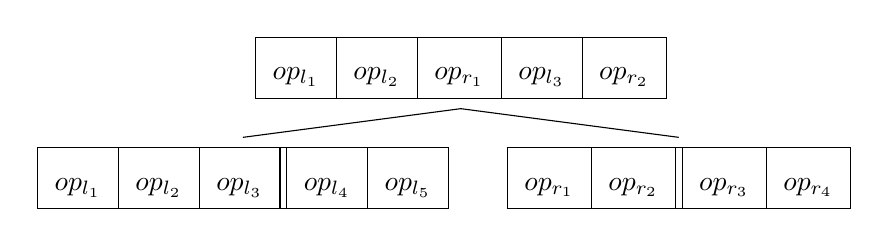
\begin{tikzpicture}[level 1/.style={level distance=1.4cm,sibling distance=0.5cm}]
\Tree [.{\begin{tabular}{|c|c|c|c|c|c|}  \hline $op_{l_1}$ & $op_{l_2}$ & $op_{r_1}$ & $op_{l_3}$ & $op_{r_2}$ \\ \hline \end{tabular}}
{\begin{tabular}{|c|c|c||c|c|}  \hline $op_{l_1}$ & $op_{l_2}$ & $op_{l_3}$ & $op_{l_4}$ & $op_{l_5}$ \\ \hline \end{tabular}}
{\begin{tabular}{|c|c||c|c|}  \hline $op_{r_1}$ & $op_{r_2}$ & $op_{r_3}$ & $op_{r_4}$\\ \hline \end{tabular}} ]
\end{tikzpicture}
}
  \caption{Operations after $||$ are new.}

\end{subfigure}
\hfill
\begin{subfigure}[b]{.49\textwidth}


  \centering
  \resizebox{\columnwidth}{!}{
  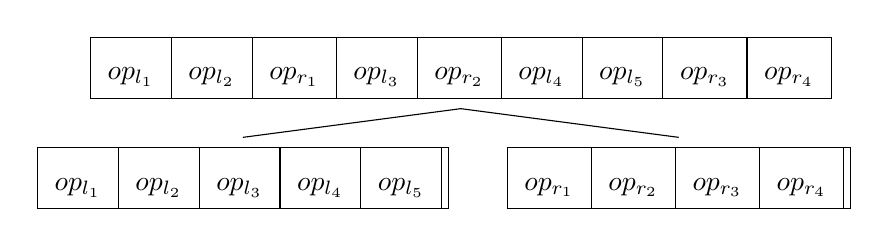
\begin{tikzpicture}[level 1/.style={level distance=1.4cm,sibling distance=0.5cm}]
\Tree [.{\begin{tabular}{|c|c|c|c|c|c|c|c|c|c|}  \hline $op_{l_1}$ & $op_{l_2}$ & $op_{r_1}$ & $op_{l_3}$ & $op_{r_2}$ & $op_{l_4}$ & $op_{l_5}$ & $op_{r_3}$ & $op_{r_4}$  \\ \hline \end{tabular}}
{\begin{tabular}{|c|c|c|c|c||}  \hline $op_{l_1}$ & $op_{l_2}$ & $op_{l_3}$ & $op_{l_4}$ & $op_{l_5}$ \\ \hline \end{tabular}}
{\begin{tabular}{|c|c|c|c||}  \hline $op_{r_1}$ & $op_{r_2}$ & $op_{r_3}$ & $op_{r_4}$\\ \hline \end{tabular}} ]
\end{tikzpicture}
}
  \caption{New operations are added to the parent node.}

\end{subfigure}


\caption{\label{fig:ucexample} Propagate Step in Universal Construction}
\end{center}
\end{figure}


\begin{algorithm}
\caption{Universal Construction Idea}\label{alg1}
\begin{algorithmic}[1]
\begin{multicols}{2}

\Function{response}{Do}{\textsl{operation} op, \textsl{pid} i} 
\State \texttt{l\textsubscript{i}.\Call{append}{op}}
\State \Call{Propagate}{parent of l\textsubscript{i}}
\State \texttt{Run} \textsf{the sequence stored in root}
\State \texttt{\Return op}\textsf{'s response from line 4}
\EndFunction{Do}

\Statex

\Function{void}{Propagate}{\textsl{node} n}
\If{\texttt{n==root}} \Return
\ElsIf{!\Call{Refresh}{n}}
\State \Call{Refresh}{$n$} \EndIf
\State \Call{Propagate}{parent of n}
\EndFunction{Propagate}

\columnbreak

\Function{boolean}{Refresh}{\textsl{node} n}
\State \texttt{old=} \Call{Read}{n}
\State \texttt{new=} \textsf{ops that n's children contain but \texttt{old} does not}
\State \texttt{new= old$\cdot$new}
\State \Return n.\Call{CAS}{old, new}
\EndFunction{Refresh}

\end{multicols}
\end{algorithmic}
\end{algorithm}

$\textsc{O}(\log n)$ CAS operations are invoked to do a \textsc{Propagate}, but the CAS words store sequences of unbounded length.
The problem is that we are trying to store unbounded sequence of operations in each node $n$ (see Figure~\ref{fig::uc}). However, to compute the result of an operation, we only use the total ordering that is stored at the root. Although we use a similar construction for our queue implementation, we develop an implicit representation of the sequence of operations, so that we can use reasonable size CAS objects and still achieve polygarithmic step complexity.

\begin{figure}[h]
\begin{center}
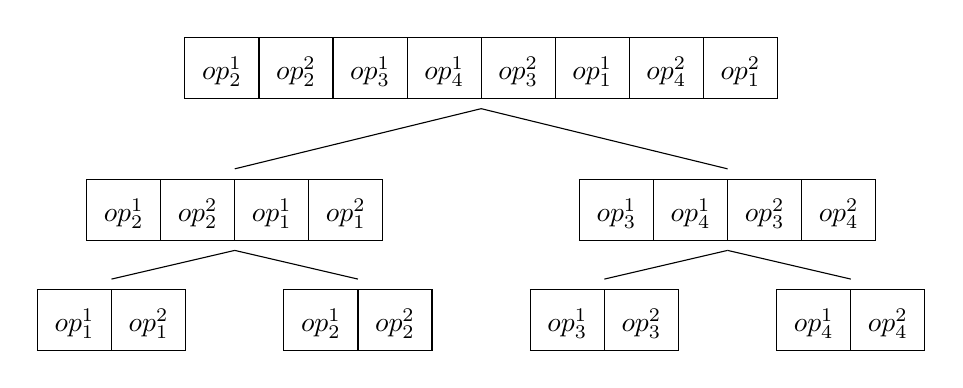
\begin{tikzpicture}[level 1/.style={level distance=1.8cm,sibling distance=1cm}, level 2/.style={level distance=1.4cm,sibling distance=1cm}]
  
\Tree [.{\begin{tabular}{|c|c|c|c|c|c|c|c|c|c}  \hline  $op_2^1$ & $op_2^2$ & $op_3^1$ & $op_4^1$ & $op_3^2$ & $op_1^1$ & $op_4^2$ & $op_1^2$ \\ \hline\end{tabular}}  [.{\begin{tabular}{|c|c|c|c|c|c}  \hline $op_2^1$ & $op_2^2$ & $op_1^1$ & $op_1^2$ \\ \hline\end{tabular}}
      {\begin{tabular}{|c|c|c|c}  \hline $op_1^1$ & $op_1^2$ \\ \hline\end{tabular}} {\begin{tabular}{|c|c|c|c}  \hline $op_2^1$ & $op_2^2$ \\ \hline\end{tabular}} ] [.{\begin{tabular}{|c|c|c|c|c|c}  \hline $op_3^1$ & $op_4^1$ & $op_3^2$ & $op_4^2$ \\ \hline\end{tabular}} {\begin{tabular}{|c|c|c|c}  \hline $op_3^1$ & $op_3^2$ \\ \hline\end{tabular}} {\begin{tabular}{|c|c|c|c}  \hline $op_4^1$ & $op_4^2$ \\ \hline\end{tabular}} ] ]

\end{tikzpicture}
\caption{\label{fig::uc} Universal Construction: $op_j^i$ denotes the $i$th operation from process $j$. In each node, we store the ordering of all the operations propagated up to it.}
\end{center}
\end{figure}

\section{Block Tree}

%\subsection{Idea in a nutshell}
We apply two ideas from universal construction to create a new linearizable data structure agreeing on a sequence of elements among processes. First, there is a shared tournament tree among processes, in which each process appends its element to its leaf in the tree and then tries to propagate it up to the root by performing \textsc{Refresh()} operations at each node. Second, each operation is linearized when its element is appended to the root.

\subsection{Sequence of propagated operations}
\paragraph{}
The basic idea behind the universal construction is to create a linearization of operations invoked by processes. If we design a fast shared data structure in which processes can append elements to a sequence, we can use it to implement practical, fast implementaion of an object $O$ by using the sequence data structure to keep track of the sequence of operations  on $O$. In the following sections, we introduce our solution called Block~Tree.

%\begin{lemma}
%    Consider an instance of \textsc{Propagate(}\textnormal{n}\textsc{)}. When it terminates all operations that were in $n$ before \textsc{Propagate(}\textnormal{n}\textsc{)} will be in the root. \texttt{(not suitable place)}
%\end{lemma}

\subsection{Sequence of Sets of Concurrent Operations \label{subsec::block}}
\paragraph{}
 In the universal construction, we order new concurrent operations at each \textsc{Refresh}() and maintain that order in the path up to the root. However, we can instead keep track of sets of concurrent operations and create the total ordering of all operations at the root (see Figure~\ref{fig::set}).
 
 \begin{figure}[h]
\begin{center}
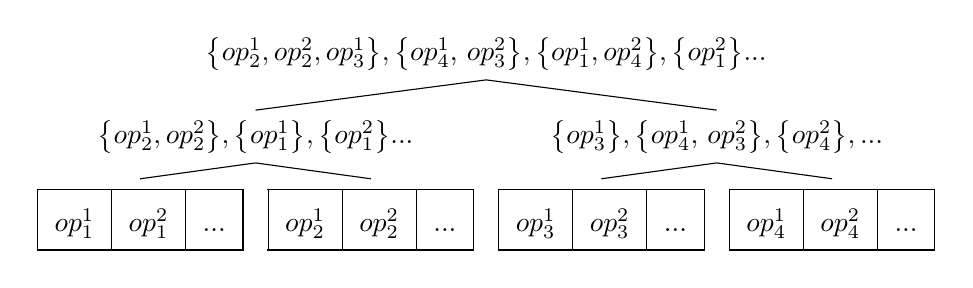
\begin{tikzpicture}
  
\Tree [.{$\big\{op_2^1,op_2^2,op_3^1\big\},\big\{op_4^1$, $op_3^2\big\},\big\{op_1^1, op_4^2\big\},\big\{op_1^2\big\}...$ }  [.{ $\big\{op_2^1, op_2^2\big\},\big\{op_1^1\big\},\big\{op_1^2\big\}...$ }
      {\begin{tabular}{|l|c|c|c}  \hline $op_1^1$ & $op_1^2$ & ... \\ \hline\end{tabular}} {\begin{tabular}{|l|c|c|c}  \hline $op_2^1$ & $op_2^2$ & ... \\ \hline\end{tabular}} ] [.{ $\big\{op_3^1\big\},\big\{op_4^1$, $op_3^2\big\},\big\{op_4^2\big\},...$ } {\begin{tabular}{|l|c|c|c}  \hline $op_3^1$ & $op_3^2$ & ... \\ \hline\end{tabular}} {\begin{tabular}{|l|c|c|c} \hline $op_4^1$ & $op_4^2$ & ... \\ \hline\end{tabular}} ] ]

\end{tikzpicture}
\caption{\label{fig::set} In each internal node, we store the set of all the operations propagated together, and one can arbitrarily linearize the sets of concurrent operations among themselves. Since we linearize operations when they are added to the root, ordering the blocks in the root is important.}
\end{center}
\end{figure}


The definition of linearizability allows concurrent operations to be reordered arbitrarily. Thus, a group of concurrent operations can be appended to our root sequence as one block without specifying the order among the operations.


%\begin{lemma}
%Operations in the same block can be linearized in any order.
%\end{lemma}

\subsection{Using arrays instead of big CAS Objects}
\paragraph{}
 We used unbounded CAS objects storing sequences as big words in the universal construction. One can represent sequences as arrays to overcome this implementation problem. Each array element will store one of the blocks of concurrent operations described in section \ref{subsec::block}.
 
\subsection{Augmenting Tree to make \textsc{Refresh}() Step faster}
\paragraph{}
Copying operation sequences from children to their parent in a \textsc{Refresh}() takes time proportioned to the number of operations being copied. This is time-consuming, so we propose a way to augment the tree to calculate lines 15,16 in $\textsc{O}(\log p)$ steps which reads new operation and concats them with old operations. Instead of representing the set of operations by explicitly listing them in a node, we represent a set of operations implicitly by recording which of the children's sets were unioned to create the set. Having operation sequences stored at leaves, we can deduce a set of operations in a node using this implicit representation.~(see Figure~\ref{fig:block}.)


\begin{figure}

\begin{center}
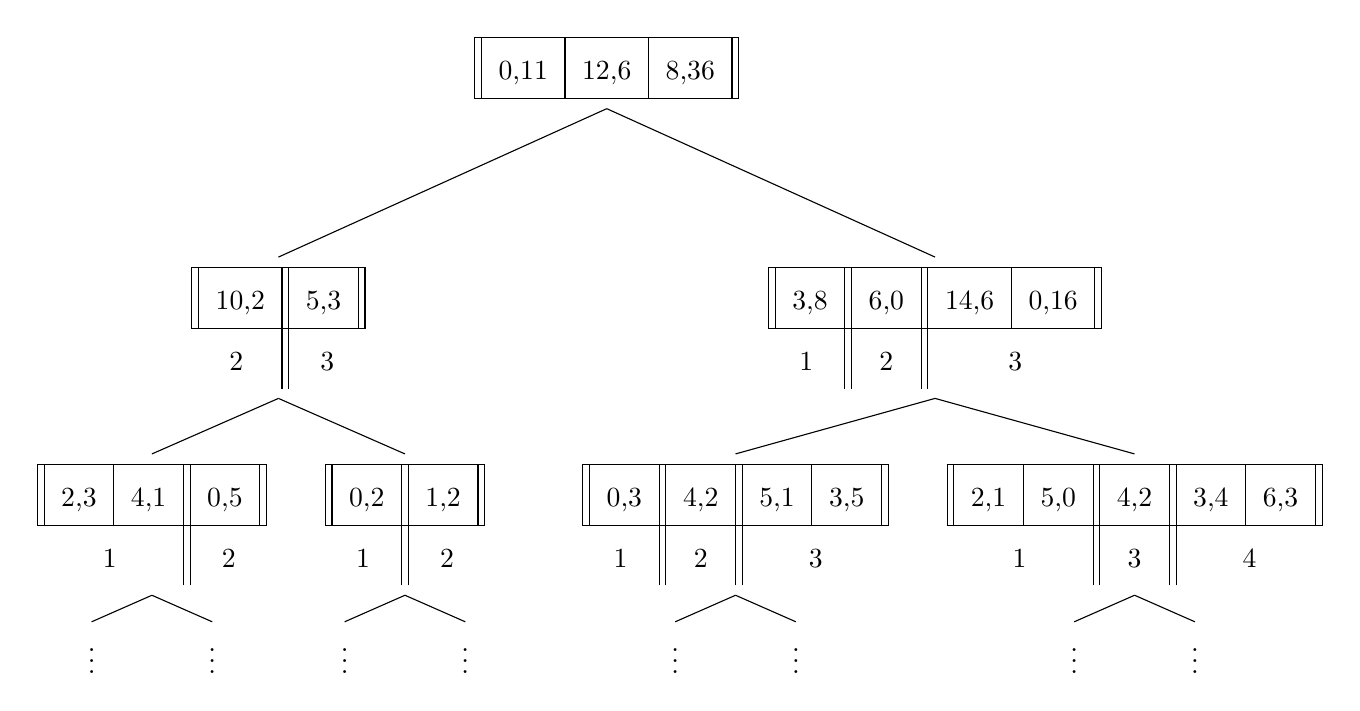
\begin{tikzpicture}[level 1/.style={level distance=3.3cm,sibling distance=1cm},
	level 2/.style={level distance=2.5cm,sibling distance=0.5cm},
	level 3/.style={level distance=1.8cm,sibling distance=1.2cm}]
  

\Tree [.{\begin{tabular}{||c|c|c||}  \hline 0,11 & 12,6 & 8,36 \\ \hline\end{tabular}}
 [.{\begin{tabular}{||c||c||}  \hline 10,2 & 5,3 \\  \hline \multicolumn{1}{c||}{2} & \multicolumn{1}{c}{3} \end{tabular}}
 [.{\begin{tabular}{||c|c||c||}\hline 2,3 & 4,1 & 0,5 \\\hline\multicolumn{2}{c||}{1} & \multicolumn{1}{c}{2}\end{tabular}} $\vdots$ $\vdots$ ]
  [.{\begin{tabular}{||c||c||}  \hline 0,2 & 1,2 \\  \hline \multicolumn{1}{c||}{1} & \multicolumn{1}{c}{2} \end{tabular}} $\vdots$ $\vdots$ ] ]
          [.{\begin{tabular}{||c||c||c|c||}  \hline 3,8 & 6,0 & 14,6 & 0,16 \\ \hline \multicolumn{1}{c||}{1} & \multicolumn{1}{c||}{2} & \multicolumn{2}{c}{3}\end{tabular}}
           [.{\begin{tabular}{||c||c||c|c||}  \hline 0,3 & 4,2 & 5,1 & 3,5 \\ \hline \multicolumn{1}{c||}{1} & \multicolumn{1}{c||}{2}& \multicolumn{2}{c}{3}\end{tabular}} $\vdots$ $\vdots$ ]
            [.{\begin{tabular}{||c|c||c||c|c||}  \hline 2,1 & 5,0 & 4,2 & 3,4 & 6,3 \\ \hline \multicolumn{2}{c||}{1} & \multicolumn{1}{c||}{3} & \multicolumn{2}{c}{4}\end{tabular}} $\vdots$ $\vdots$ ] ] ]

\end{tikzpicture}
\end{center}
\caption{\label{fig:block} Showing concurrent operation sets with blocks. Each block consists of a pair(left, right) indicating the number of operations from the left and the right child, respectively. Block (12,6) in the root contains blocks (10,2) from the left child and (6,0) from the right child. Blocks between two lines $||$ are propagated together to the parent. For example, Blocks (2,3) and (4,1) from the leftmost leaf and (0,2) from its sibling are propagated together into the block (10,2) in their parent. The number underneath a group of blocks in a node indicates which block in the node's parent those blocks were propagated to.}
\end{figure}


Each block $b$ in node $n$ is the aggregation of blocks in the  children of $n$ that are newly read by the\textsc{Propagate}() step that created block $b$. For example, the third block in the root (8,36) is created by merging block (5,3) from the left child and (14,6) and (0,16) from the right child. Block (5,3) also points to elements from blocks (0,5) and (1,2). 
%Recursively we can deduce each block contents until the leaf nodes store arrays of individual element operations.

\begin{definition}\{Existence of an operation in a block\}  Operation op exists in block b if it has propagated up to block b.
\end{definition}


\begin{definition}\{Subblock\}
  The blocks that are aggregated into block $b$ in a \textsc{Propagate}() step are called subblocks of $b$. Block $b_1$ is a subblock of $b_2$ if and only if $b_1$ is a block in node $v$ and in $b_2$ is a block in the parent of $v$ and $b_1$'s elements exits in $b_2$'s elements.
\end{definition}
%{\TODO: describe how blocks work with a good example how exactly it is done}

\paragraph{}
We choose to linearize operations from the left child before those from the right child as a convention. In effect, this means that if there are concurrent operations in a \textsc{Refresh}() step from several processes we linearize them in the order of their process ids. So for example  operations aggregated in block (10,2) are in the order (2,3),(4,1),(0,2). All blocks from the left child with come before the right child and the order of blocks of each child is preserved among themselves.
%\begin{lemma}
%\label{lem:block_size}
%There cannot be more than one operation from each process in a \textsc{Refresh}() invocation.
%\end{lemma}
%\begin{proof}
%  If so, then that parent process has invoked two simultaneous operations. $ \blacksquare $
%\end{proof}

\paragraph{}
In a \textsc{Propagate}() invocation path from a leaf to root, there will be \textsc{Refresh}() steps with merges from $2, 4, 8, ..., p$ processes. So in a complete propagation, at most $2p$ blocks are merged into one block. \texttt{(maybe useful for analysis)}
%\begin{lemma}
%A block in the root cannot contain more than one operation from a process.
%\end{lemma}
%\begin{proof}
%  Assume a process in a block invokes two operations; one has to be finished another. If so, it has been added to root before. $\blacksquare$
%\end{proof}

\subsection{Using pointers and prefix sum to make \textsc{GetIndex}($i$) faster}
%\begin{definition}
%  \textsc{BSearch}($i$): Search $i$th element in a prefix sum array with length $n$ in \textsc{O}($\log n$) steps.
%\end{definition}
\paragraph{}
\textsc{GetIndex}($i$) returns the $i$th operation stored in the block tree sequence. We do that by finding the block $b_i$ containing $i$th element in the root, and then recursively finding the subblock of $b_i$ which contains $i$th element. To make this recursive search faster, instead of iterating over all elements in sequence of blocks we store prefix sum of number of elements in the blocks sequence and pointers to make BSearch faster.

Furthermore, in each block, we store the prefix sum of left and right elements. Moreover, for each block, we store two pointers to the last left and right subblock of it (see fig \ref{fig::pointer} and \ref{fig:prefix}).

\begin{figure}
\begin{center}
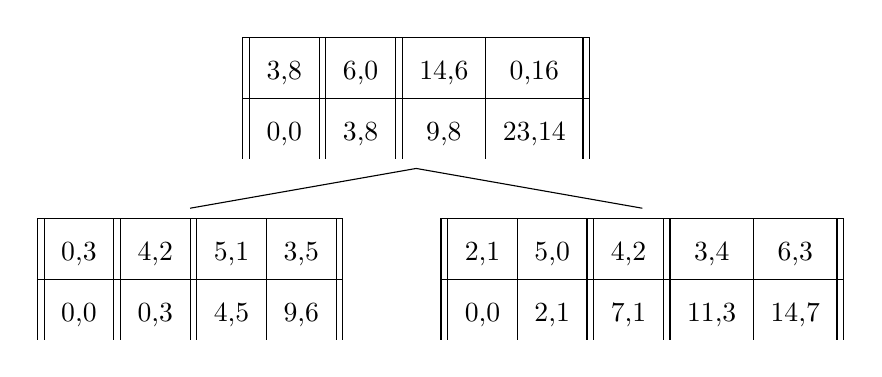
\begin{tikzpicture}[level 1/.style={level distance=2.3cm,sibling distance=1cm}]
  
\Tree [.{\begin{tabular}{||c||c||c|c||}  \hline 3,8 & 6,0 & 14,6 & 0,16 \\ \hline  0,0 & 3,8 & 9,8 & 23,14\end{tabular}}
           [.{\begin{tabular}{||c||c||c|c||}  \hline 0,3 & 4,2 & 5,1 & 3,5 \\ \hline 0,0 & 0,3 & 4,5 & 9,6 \end{tabular}} ]
            [.{\begin{tabular}{||c|c||c||c|c||}  \hline 2,1 & 5,0 & 4,2 & 3,4 & 6,3 \\ \hline 0,0 & 2,1 & 7,1 & 11,3 & 14,7 \end{tabular}} ] ]


\end{tikzpicture}
\end{center}
\caption{\label{fig:prefix} Using Prefix sums in blocks. When we want to find block b elements in its children, we can use binary search. The number below each block shows the count of elements in the previous blocks.}
\end{figure}

\begin{figure}[hbt]
\centering
  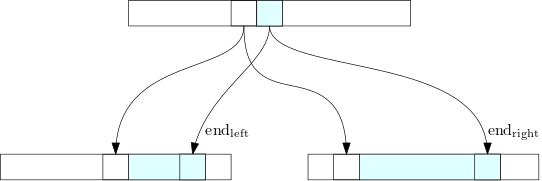
\includegraphics[width=5in]{pics/pointers}
  \caption{Block have pointers to the starting block of theirs for each child. \label{fig::pointer}}
\end{figure}

\paragraph{}
Starting from the root, \textsc{GetIndex}($i$) BSearches $i$ in the prefix sum array to find block containing $i$th operation, then continues recursively calling \textsc{GetElement}($b,i$) to find $i$th element of block $b$. From lemma $\ref{lem:block_size}$ we know a block size is at most $p$. So BSearch takes at most \textsc(O)$(\log p)$, since  with knowing pointers of a block and its previous block we can determine the base \texttt{(domain ?)} to search and its size is \textsc{O}$(p)$.

\subsection{Block Tree Algorithm}
\paragraph{}
Our Block Tree is a linearizable implementation of a data structure that stores the elements appended by processes. It has two methods (see Algorithm~\ref{alg2}), \textsc{Append}($e$) which appends element $e$ to the sequence, and \textsc{GetIndex}($i$) which returns the $i$th element in the sequence.

\paragraph{Design of a block tree}

Each process is assigned with a leaf in a shared tournament tree. Thus, for example, the leaf node for process $p_i$ contains an array of operations by $p_i$ in the order they were invoked.
Each internal node of the tree contains an array of blocks of elements.
Block $b$ in node $n$ is created in a \textsc{Propagate}() step and is merged block of new blocks at the time of \textsc{Propagate}() reading $n$'s children blocks. Each block consists of pointers left and right, to the last block merged into itself from left and right child in that order. Moreover, two numbers, left, right indicating the count of elements in the blocks from left and right child consecutively. Furthermore, two amounts, prefix left and prefix right, can be computed from the prefix sum of left and right values.
Elements of block $b$ can be determined recursively (\textsc{GetElements($b$)}).
Element $i$th in the sequence can be determined in \textsc{O}($\log^2 p$) steps by recursively finding $i$th element in block $b$ (\textsc{GetElement($i$)})
After element $e$ is propagated (appended to a block int the root), its index can be computed with \textsc{GetIndex}($op$).


In order to compute elements of a block faster we store prefix-sum blocks(block i has tuple(right-sum=$\#$right ops in previous block, left-sum=$\#$left ops in previous blocks)[See Figure \ref{fig:prefix}]. Here is the algorithm to get elements of a block.


\begin{algorithm}
\caption{Block Tree \label{alg2}}
\begin{algorithmic}[1]
\begin{multicols}{2}

\Statex \textbf{Structure}

\Statex $\blacktriangleright$ \texttt{\textsl{operation} op}
\begin{itemize}
\item \texttt{\textsl{string} name}
\item \texttt{\textsl{int} pid}
\item \texttt{\textsl{int} loc \textsf{: location in leaf's array}}
\end{itemize}


\Statex $\blacktriangleright$ \texttt{\textsl{leaf} l\textsubscript{i}}
\begin{itemize}
\item \texttt{\textsl{*node} parent} \textsf{: pointer to parent in Tree}
\item \texttt{\textsl{operation[]} ops} \textsf{: ops invoked by process i}
\item \texttt{\textsl{int} last= 1} \textsf{: index of first empty cell of \texttt{ops}}
\end{itemize}


\Statex $\blacktriangleright$ \texttt{\textsl{node} n}
\begin{itemize}
\item \texttt{\textsl{*node} left, right, parent}
\item \texttt{\textsl{block[]} blocks} \textsf{: blocks propagated to \texttt{n}}
\item \texttt{\textsl{int} last= 1} \textsf{: index of first empty cell of \texttt{blocks}}
\end{itemize}



\Statex $\blacktriangleright$ \texttt{\textsl{block} b}
\begin{itemize}
  \item \texttt{\textsl{int} num\textsubscript{left}, num\textsubscript{right}, sum, sum\textsubscript{left}, sum\textsubscript{right}} \textsf{:~\#~operations from the left and the right child, sum of all operations, prefix sum of operations from the left and the right child}
  \item \texttt{\textsl{int} end\textsubscript{left}, end\textsubscript{right}} \textsf{: index of \texttt{b}'s last subblock}
\end{itemize}


\Statex \textbf{Examples}
\Statex \hspace{0pt} \texttt{ l\textsubscript{i}[j]}\textsf{: jth operation of ith process}
\Statex \hspace{0pt} \texttt{ n.left}\textsf{: left child of node n}
\Statex \hspace{0pt} \texttt{ n.blocks[n.last]}\textsf{: index of last block of node n}
\Statex \hspace{0pt} \texttt{ n.blocks[i].num\textsubscript{left}}\textsf{: \#left operations of ith block of n}
\Statex \hspace{4pt} \texttt{b.end\textsubscript{right}}\textsf{: ending right subblock of b position}

\Statex

\Function{int}{Append}{\textsl{operation} op, \textsl{int} pid} 
\State \texttt{op.loc= l\textsubscript{pid}.last + 1}
\State \texttt{l\textsubscript{pid}.ops[op.location]= op}
\State \Call{Propagate}{l\textsubscript{pid}.parent}
\State \Return \Call{Index}{l\textsubscript{pid}, op.location}
\EndFunction{Append}

\columnbreak

\Function{element}{Get}{\textsl{int} i} 
\State \texttt{res=\Call{BSearch}{root, sum, i, 0, root.last}}
\State \Return{\Call{Get}{root, res, i-root.blocks[res-1].sum}}
\EndFunction{Get}

\Statex

%\Function{index}{Index}{operation op, int pid}
%\State \texttt{\textsl{int} i= op's order in l\textsubscript{pid}.ops}
%\State \Return \Call{Index}{l\textsubscript{p}, i}
%\EndFunction{Index}

%\Statex

\Function{void}{Propagate}{\textsl{node} n}
\If{\texttt{n {\keywordfont is} root}} \Return
\Else
\State \texttt{i= n.last}
\State \texttt{\textsl{block} new=\Call{CreateBlock}{n, i+1}}
\If{\Call{CAS}{n.blocks[i+1], null, new}}
\State \texttt{\Call{CAS}{n.last, i, i+1}}
\Else
\State \texttt{i= n.last}
\State \texttt{\textsl{block} new=\Call{CreateBlock}{n, i+1}}
\If{\Call{CAS}{n.blocks[i+1], null, new}}
\State \texttt{\Call{CAS}{n.last, i, i+1}}
\EndIf
\EndIf
\EndIf
\State \Call{Propagate}{n.parent}
\EndFunction{Propagate}

\Statex

\Function{block}{CreateBlock}{\textsl{node} n, \textsl{int} i} 
\Statex\Comment{Creates a block to insert into \texttt{n.blocks[i]}}
\State \texttt{block b= \Call{new}{\textsl{block}}}
\ForEach{\texttt{dir} {\keywordfont{in}} \texttt{\{left, right\}}}
\State \texttt{prev= n.blocks[i-1].ending\textsubscript{dir}}
\State \texttt{j= n.dir.last}
\State \texttt{end= n.dir.blocks[j]}
\State \texttt{b.end\textsubscript{dir}= j}
\State \texttt{b.num\textsubscript{dir}= end.sum\textsubscript{\#dir} - start.sum\textsubscript{\#dir}}
\State \texttt{b.sum\textsubscript{\#dir}= n.blocks[i-1].sum\textsubscript{\#dir} + b.num\textsubscript{dir}}
\EndFor
\State \texttt{b.sum= b.sum\textsubscript{left} + b.sum\textsubscript{right}}
\State \Return \texttt{b}
\EndFunction{CreateBlock}




\end{multicols}
\end{algorithmic}
\end{algorithm}

\begin{algorithm}
\caption{Block Tree Continued}
\begin{algorithmic}[1]

\Statex

\Statex $\leadsto$ \textsf{Precondition: \texttt{n.blocks[start..end]} contains a block with feild \texttt{f} $\geq$ \texttt{i}}
\Function{int}{BSearch}{\textsl{node} n, \textsl{field} f, \textsl{int} i, \textsl{int} start, \textsl{int} end}

\Statex \Comment{\textmd{Searches~the value \texttt{i} of the given prefix sum \texttt{type} on the node \texttt{n} in the domain from \texttt{start} to \texttt{end} blocks. \texttt{f} is one of \texttt{sum, sum\textsubscript{left}, sum\textsubscript{right}}. Does binary search on \textsl{field} \texttt{f} of the blocks stored in \texttt{n.blocks} and returns the index of the leftmost block in \texttt{n.blocks[start..end]} whose \textsl{field} \texttt{f} is $\geq$ \texttt{i}}.}
\State \Return \texttt{result block's index}
\EndFunction{BSearch}

\Statex

\Function{element}{Get}{node n, int b, int i} 
\Comment{\textmd{Returns the \texttt{i}th operation in \texttt{b}th block of node \texttt{n}}}

\If{\texttt{i $\leq$ b.num\textsubscript{left}+1}} \Comment{\texttt{i} exists in left child of \texttt{n}}
\If{\texttt{n.left {\keywordfont is} leaf}} \Return \texttt{n.left.ops[i]}
\Else
\State \texttt{subBlock= \Call{BSearch}{n.left.sum, i, n.blocks[b-1].end\textsubscript{left}+1, n.blocks[b].end\textsubscript{left}}}
\State \Return\Call{Get}{n.left, subBlock, i-n.left.blocks[subBlock-1].sum} 
\EndIf
\Else
\State \texttt{i= i-n.blocks[b].sum\textsubscript{left}}
\If{\texttt{n.right {\keywordfont is} leaf}} \Return \texttt{n.right.ops[i]}
\Else 
\State\texttt{subBlock=\Call{BSearch}{n.right.sum, i, n.blocks[b-1].ending\textsubscript{right}, n.blocks[b].ending\textsubscript{right}}}
\State \Return\Call{Get}{n.right, subBlock, i-n.right.blocks[subBlock-1].sum} \EndIf
\EndIf
\EndFunction{Get}

\Statex

\Function{index}{Index}{node n, int i} \Comment{Returns order in root of \texttt{i}th operation in node \texttt{n}}
\If{\texttt{n {\keywordfont is} root}} \Return \texttt{i}
\Else
\State \texttt{nBlock= \Call{BSearch}{n, n.sum, i, 0, n.parent.last}}
\Comment{\textmd{This search takes O(log n) steps}}
\State \texttt{dir= (n.parent.left==n)?left:right}
\State \texttt{superBlock= \Call{BSearch}{n.parent, n.sum\textsubscript{dir}, i, 0, n.parent.last}}
\Comment{\textmd{This search takes O(log n) steps}}
\If{\texttt{dir {\keywordfont is} left}}
\State \texttt{i+= n.parent.blocks[superBlock-1].sum + n.blocks[nBlock-1].sum}
\Else \State \texttt{i+= n.parent.blocks[superBlock-1].sum + n.parent.blocks[superBlock].sum\textsubscript{left} + n.blocks[nBlock-1].sum}
\EndIf
\State \Return\Call{Index}{n.parent,}
\EndIf
\EndFunction{Index}

\Statex

%\Function{list}{GetElements}{block b} 
%\ForEach{block {\keywordfont in} \Call{GetSubBlocks}{b}}
%\State result.append(\Call{GetElements}{})
%\EndFor
%\State \Return result
%\EndFunction{GetElements}
%
%\Statex
%
%\Function{list}{GetSubBlocks}{b}
%\State n:=b.node
%\State b[-1]=b's previous block
%\ForEach{direction \{left, right\}}
%\State init=\Call{BSearch}{n.direction, b[-1].direction}
%\State end=\Call{BSearch}{n.direction, b.direction}
%\State result.append([init:end])
%\EndFor
%\State \Return result
%\EndFunction{GetSubBlocks}

\end{algorithmic}
\end{algorithm}

\section{Implementing Queue using Block Tree}
\subsection{Idea in a nutshell}
With the ideas introduced in block tree we are going to create a shared wait-free queue with \textsc{O}$(\log p)$ steps. A queue consitsts of two operations, enqueue and dequeue. \textsc{Enqueue}$(n)$ appends element $n$ to the sequence stored, this is somehow similar to \textsc{Append}$(n)$. Since \textsc{Append}$(n)$  adds $n$ to the history of all operations. \textsc{Dequeue()} returns first not dequeued element among all elements. If index $i$ is the tail of the queue, we can return the dequeue response using \textsc{GetElement}$(i)$.  So in the rest we modify block tree to compute $i$ for each \textsc{Dequeue}$()$ to achieve a FIFO queue.

\subsection{What should a \textsc{Dequeue}$()$ return, regarding history of operations?}
\paragraph{}
In a basic look of we use block tree to implement queues the block tree, we maintain the sequence of all elements(history of all operations), not only the current state of the queue. Regarding the current state of the queue, if it is not empty, the \textsc{Dequeue}$()$ returns the first existing element. And if the queue is empty it returns \texttt{null}. Now look at all the history of operations, what should $i$th \textsc{Dequeue}$()$ return?

\begin{table}[hbt]
\centering
  \begin{tabular}{c|c|c|c|c|c|c|c|c|c}
    \hline \texttt{ENQ(5)}& \texttt{ENQ(2)}& \texttt{DEQ()}& \texttt{ENQ(3)}&\texttt{DEQ()}& \texttt{DEQ()}& \texttt{DEQ()}& \texttt{ENQ(4)}& \texttt{ENQ(6)}& \texttt{DEQ()}\\ \hline
  \end{tabular}
  \caption{An example histoy of operations on the queue}
\end{table}

\paragraph{}
In the example above, \textsc{Dequeue}$()$ operations return \texttt{5, 2, 3, null, 4} in order. If the queue size is greater than $0$ and $r$ Dequeue operations have returned a non-null response, then $i$th Dequeue returns $r+1$th Enqueue input. So in order to answer a Dequeue, there is only needed to know the size of the queue and $\#$ returning dequeues.

\texttt{DEQ[i] = (size>0) ? ENQ[r+1] : null;}
\begin{definition}
After a sequence of operations, $\#$returning dequeues is the number of Dequeue operations that have returned non null value. \texttt{DEQ[i]} is the $i$th Dequeue. \texttt{ENQ[i]} is the argument of $i$th Enqueue.
\end{definition}

\subsection{What should a \textsc{Dequeue}$()$ return, regarding history of blocks of operations?}

\paragraph{}
In the Block Tree idea, we did not store the sequence of operations themselves but instead stored blocks of concurrent operations to optimize \textsc{Propagate()} steps and increase parallelism. So now the problem is to find \texttt{ENQ[j]} for \texttt{DEQ[i]}. From lemma \ref{lem:block_size} we know we can linearize operations in a block in any order; here, we choose to decide to put Enqueue operations in a block before Dequeue. In the next example, operations in a cell are concurrent, and the order within a block is as said before. \texttt{DEQ()} operations return \texttt{null, 5, 2, 1, 3, 4 , null} respectively.

\begin{table}[hbt]
\centering
  \begin{tabular}{c|c|c|c}
    \hline \texttt{DEQ()} & \texttt{ENQ(5)}, \texttt{ENQ(2)}, \texttt{ENQ(1)}, \texttt{DEQ()}& \texttt{ENQ(3)}, \texttt{DEQ()}&  \texttt{ENQ(4)}, \texttt{DEQ()}, \texttt{DEQ()}, \texttt{DEQ()}, \texttt{DEQ()}\\ \hline
  \end{tabular}
  \caption{An example histoy of operation blocks on the queue}
\end{table}

\paragraph{}
In the last section, we claimed that by knowing the current size of the queue and $\#$returning dequeue operations before the current state, we could decide the index of result Enqueue. Now we apply this information to blocks; if we store the size of the queue after a block happens and the number returning dequeues in a block, we can compute every dequeue result in \textsc{O}$(1)$ steps.

\begin{table}[hbt]
\centering
  \begin{tabular}{c|c|c|c|c}
    \hline &\texttt{DEQ()} & \texttt{ENQ(5)}, \texttt{ENQ(2)}, \texttt{ENQ(1)}, \texttt{DEQ()}& \texttt{ENQ(3)}, \texttt{DEQ()}&  \texttt{ENQ(4)}, \texttt{DEQ()}, \texttt{DEQ()}, \texttt{DEQ()}, \texttt{DEQ()}\\ \hline
    size & 0 & 2 & 2 & 0 \\ \hline
    \#enqs & 0 & 3 & 1 & 1 \\ \hline
        \#deqs & 1 & 1 & 1 & 4 \\ \hline
            \#redqs & 0 & 1 & 1 & 3 \\ \hline
  \end{tabular}
  \caption{Augmented histoy of operation blocks on the queue}
\end{table}

\begin{definition}
  \texttt{index(op)}: index of the given Dequene among same type operation in conataing block.
  
  \texttt{INDEX(op)}: index of the given Dequene among same type operation in all operations.
  
\end{definition}

Given \texttt{DEQ} is in block \texttt{b}, \texttt{response(DEQ)} would be:\\
\texttt{(size[b-1]-index(DEQ)>=0) ? ENQ[INDEX(RDEQ)+index(DEQ)] : null;}

\section{Main Algorithm}
\paragraph{}
Now that we know how to augment Block Tree root history to compute the response, we will present the complete algorithm.

\section{Time Complexity}


\bibliographystyle{abbrv}
\bibliography{main}

\end{document}